\section{Use in engineering calculations}
\label{sec:applications}
\subsection{A local two-liquid settler optimization}
% P:applications-01
A water/ethanol/isobutanol/NaCl settler connects the equilibrium and action calculations to an equation-oriented process model.
At 293.15~K and 100~kPa, the external IDAES/Pyomo model~\citep{leeIDAESProcessModeling2021,hartPyomoModelingSolving2011} minimizes normalized isobutanol and salt use subject to at least 96.5\,\% ethanol recovery in the organic outlet.
The isobutanol and salt feed rates, as multipliers of their base values, are bounded from 0.85 to 1.15, and every property call stays on a declared local two-liquid branch with Khudaida source parameters~\citep{Khudaida2026}.
The compiled external functions return outlet species amounts and exact first and second feed derivatives from the common native equilibrium equations.
The outer process optimizer therefore receives the response of the full phase split, rather than a derivative at frozen phase composition.

% P:applications-02
Three starts converge to the same local process point, with the isobutanol feed raised to 1.0604 and the salt feed lowered to 0.9152 of their base values, a normalized objective of 1.97564 against 2 at the base design, and ethanol recovery at the specified constraint.
The largest stored stationarity norm is $3.666\times10^{-12}$, complementarity is below $9.10\times10^{-11}$ and component closure below $1.12\times10^{-16}$~mol/s.
All 1\,050 transported values and derivative entries equal the native values exactly.
Figure~\ref{fig:engineering} shows the outlets and the stored local stationarity values for this same calculation.
Transport equality tests the external-function connection; balance and optimality residuals test the solved model.
The calculation is nonreactive and fixed in temperature and pressure, so it supplies neither reactive extraction validation nor a global process optimum.

\begin{figure}[pos=H]
\centering
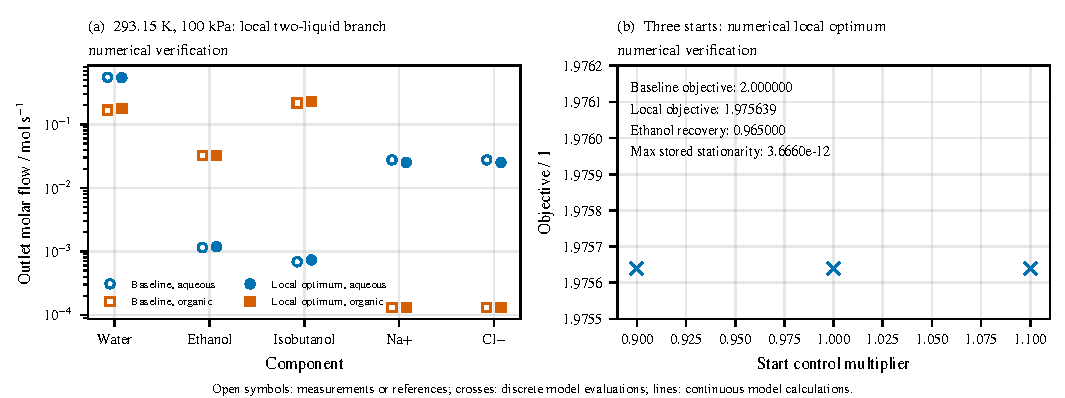
\includegraphics[width=0.96\linewidth]{F17-settler}\par
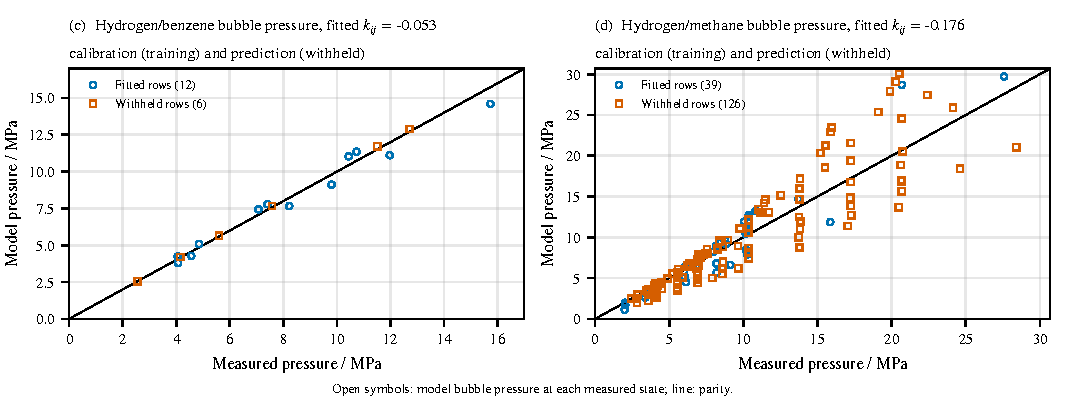
\includegraphics[width=0.96\linewidth]{F18-hda-hydrogen-pairs}
\caption{Engineering examples expose both numerical integration and parameter-domain limits.
Top: the fixed-condition Khudaida settler calculation shows outlet flows and local stationarity for the selected three-start calculation (numerical verification)~\citep{Khudaida2026}.
Bottom: hydrogen/benzene and hydrogen/methane bubble-pressure calibration and withheld prediction for pair parameters used in a two-flash example~\citep{Park1996,Benham1957,Sagara1972,Hong1981}.
}
\label{fig:engineering}
\end{figure}

\subsection{Hydrogen binary fits for a two-flash calculation}
% P:applications-03
A hydrodealkylation two-flash example uses hydrogen, methane, benzene and toluene to connect fitted pair parameters to an external phase-equilibrium model.
The external IDAES model owns its flash and smoothing equations, while the package supplies pressure-specified density, total enthalpy and component fugacity coefficients with exact derivatives.
Before any process result is interpreted, the hydrogen pair interactions must be supported by measured binary states at the conditions used.
Figure~\ref{fig:engineering} compares hydrogen/benzene and hydrogen/methane bubble pressures under zero and fitted pair interactions, with training and withheld states separated.

% P:applications-04
The hydrogen/benzene fit uses the measurements of Park et al.~\citep{Park1996}, with 12 training states at 323.2--423.2~K and six withheld states at 373.2~K.
Their bubble-pressure AARDs after fitting are 6.03\,\% and 1.20\,\%.
Hydrogen/methane uses Benham--Katz and Sagara training observations~\citep{Benham1957,Sagara1972} and Hong--Kobayashi withheld observations~\citep{Hong1981}: 39 training states at 103.15--173.65~K and 126 withheld states at 108.13--183.12~K, giving 13.9\,\% and 16.8\,\% AARD.
The fitted interactions improve the declared binary objective, but the remaining methane discrepancy is large.
The fit's discrepancy allowances and profile bands are not statistical uncertainty intervals.
Hot process states outside the binary measurement domains remain extrapolations, so numerical process convergence cannot establish their physical accuracy.



% P:applications-05
Application-specific chemistry, transport laws, parameter adoption and measured process performance require separate evidence.
The examples here demonstrate how an external model consumes the package calculations and how physical comparison limits accompany those calculations into engineering use.
They do not establish absorber performance, MEA property accuracy or lithium extraction selectivity.
